\documentclass[a4paper,11pt]{report}
\usepackage[T1]{fontenc}
\usepackage[utf8]{inputenc}
\usepackage{lmodern}
\usepackage[francais]{babel}
\addto{\captionsfrench}{\renewcommand{\abstractname}{Introduction}}
%\usepackage[top=2cm,left=2.2cm,right=2.2cm,bottom=2cm]{geometry} % Géométrie de la page, modifier selon le besoin
\usepackage{lmodern, wrapfig, textcomp, tikz, graphicx, amsmath, tikz-qtree, xcolor,rotating,epic,eepic}
\usepackage[colorlinks,linkcolor=black, urlcolor=blue]{hyperref}
\usepackage[babel=true,kerning=true]{microtype}
\usepackage{url}
\usepackage{caption}
\usepackage{subcaption}
\usepackage{array}
\date{}
\title{}
\author{}

\begin{document}
\nocite{*}
\pagenumbering{gobble}  % Pas de numérotation
\begin{titlepage}
    \vspace*{-10px}
    
\includegraphics[height=80px]{Images/logo_phelma.pdf}
    \vspace*{-80px}
\begin{flushright}
    \vspace*{-30px}
    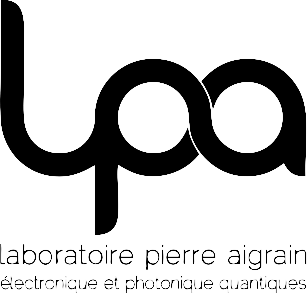
\includegraphics[height=100px]{Images/logo_lpa.png}
\end{flushright}

\vspace*{0.5cm}
\begin{center}
\rule{\linewidth}{0.5mm}\\[0.4cm]
{\huge{\bfseries Rapport de Stage d'Application}\\[0.4cm]
Mise en place d'une expérience à très basse température et étude d'effets quantiques dans des systèmes nanométriques\\[0.4cm]}
\rule{\linewidth}{0.5mm}\\[0.5cm]

\LARGE{\textsc{Félix Piédallu}}\\[0.7cm]
\large{\textsc{Filière PNS 2014-2015}}\\[2cm]

\Large{Au sein de l'équipe HQC}\\[1cm]

\includegraphics[width=0.4\textwidth]{Images/logo_HQC.pdf}\\[1cm]

\large{Sous la direction de Takis \textsc{Kontos} et Laure \textsc{Bruhat}}\\[2cm]


\end{center}
\end{titlepage}

\tableofcontents        % Table des matières avec liens, générée automatiquement.
\newpage
\pagenumbering{arabic}  % Numérotation de retour !


% Remerciements
\vspace*{\stretch{1}}
\begin{center}
\textsc{\Large Remerciements}
\\
\vspace{0.5cm}
Je tiens à remercier Takis Kontos et Laure Bruhat pour m'avoir accueilli au sein de l'équipe HQC, ainsi que pour m'avoir encadré durant ce stage. De plus, je souhaite remercier l'ensemble des membres de l'équipe avec lesquels j'ai pu échanger sur leurs projets de recherche. Enfin, je souhaite remercier Phelma Grenoble-INP pour m'avoir donné l'opportunité de réaliser ce stage.
\end{center}
\vspace*{\stretch{3}}

\chapter*{Hybrid Quantum Circuits}
L'équipe HQC fait partie du Laboratoire Pierre Aigrain, le laboratoire de l'ENS Ulm spécialisé dans la physique de la matière condensée et la physique mésoscopique.

Basé à Paris, il regroupe autour de Takis Kontos et Audrey Cottet plusieurs doctorants : Matthieu Baillergeau, Matthieu Desjardins, Matthieu Dartiailh et Laure Bruhat, avec qui j'ai essentiellement travaillé durant mon stage.

Les sujets de recherche sont essentiellement concentrés autour du transport quantique dans des nanotubes de carbone.
%TODO remplir ce paragraphe

\chapter*{Introduction} % Contexte du stage
\addcontentsline{toc}{chapter}{Introduction}

\chapter{Le cryostat à dillution}

\chapter{Le câblage DC et RF}

\chapter{Les résultats de l'expérience (avant et/ou après câblage)}


\chapter*{Conclusion}
%\input{6.Conclusion}

\bibliographystyle{unsrt}
\bibliography{bibliographie}
\end{document}
